\subsection{Hadronic Calorimeter}
\label{ild:sec:HCAL}
%\writer{Felix Sefkow, Imad Laktineh}{4}
%\textit{AHCAL beamtest results from large technological prototype, CMS HGCAL spinoff.}

\subsubsection{Scintillator option (AHCAL)}

A CALICE AHCAL physics prototype had been built and operated in 2006-2011, allowing to demonstrate the particle flow~\cite{Adloff:2011ha} and energy resolution performance~\cite{Adloff:2012gv} of the scintillator SiPM ("SiPM-on-Tile") technology for the DBD. In subsequently published papers~\cite{Adloff:2013vra,Adloff:2013kio,Adloff:2013jqa,Adloff:2014rya,Bilki:2014bga,Lucaci-Timoce:2013tkf,Price:2016sce} the adequate modelling of instrumental effects and shower evolution has been further established, and the hadronic energy resolution and linearity of a combined system with a scintillator tungsten ECAL in front was shown~\cite{Repond:2018flg} to be as good as that of the AHCAL alone, see Fig.\ref{fig:ahcal-linres}. The software used to model the detector effects such as photo-electron statistics in the SiPM has been validated by the test beam data and is also used in ILD, after adjusting for a small difference in sampling fraction only~\cite{Hartbrich:2016bbz}.
\begin{figure}[hbt]
\centering
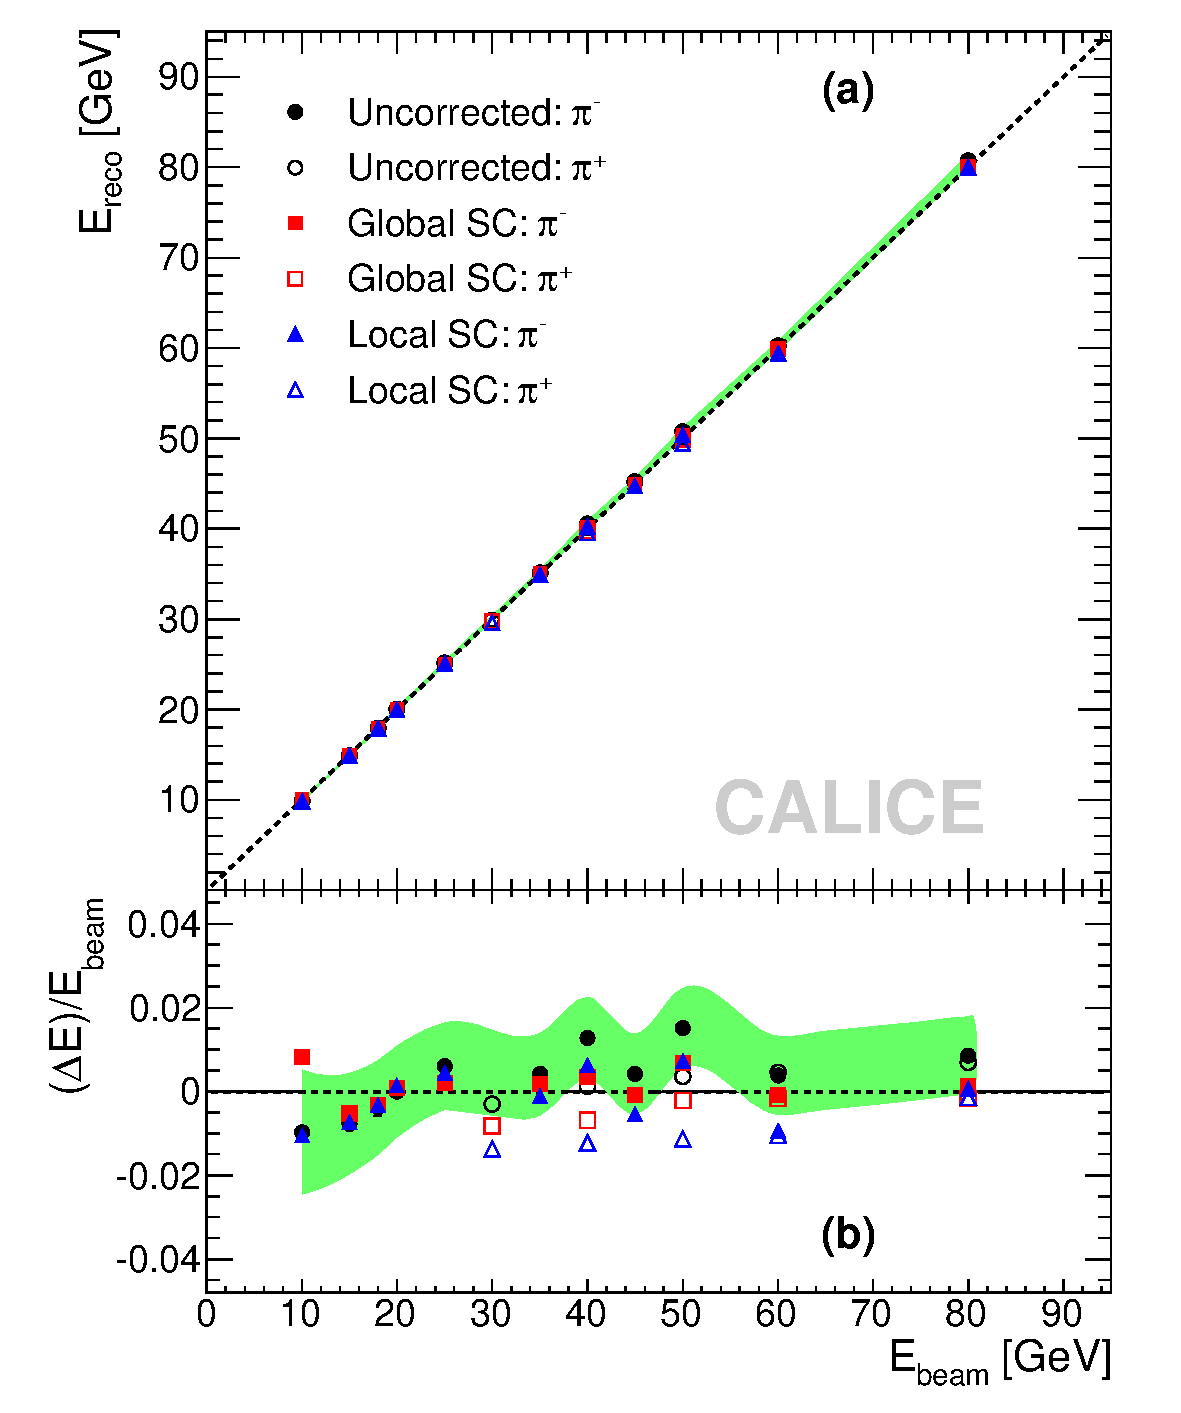
\includegraphics[width=0.39\textwidth]{Detector/fig/AHCAL-Linearity_Ini_GC_LC.pdf}
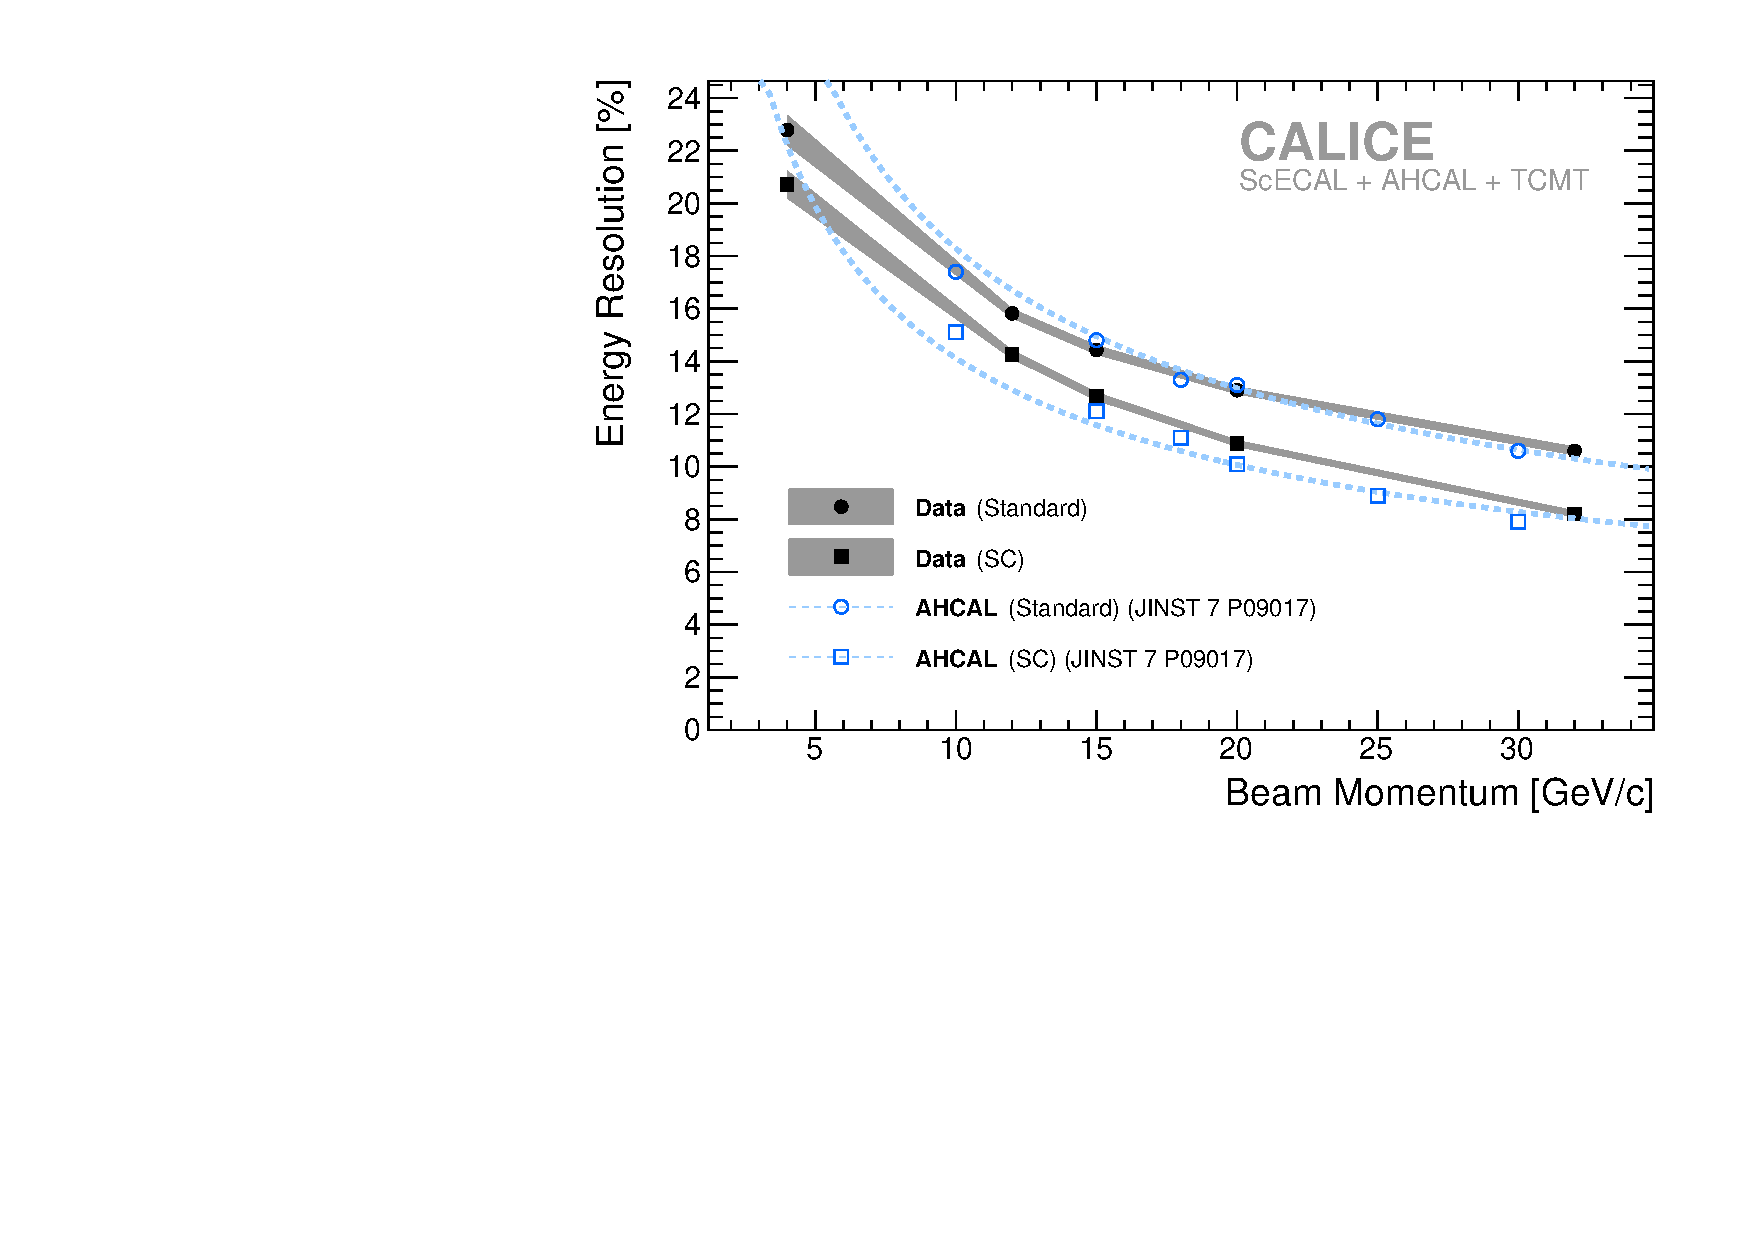
\includegraphics[width=0.59\textwidth]{Detector/fig/AHCALpion_resolution_data_ahcaljinst.pdf}
\caption{Performance of the CALICE AHCAL physics prototype for pions. Left: Response without and with global or local software compensation for the AHCAL alone (with tail-catcher, from~\cite{Adloff:2012gv}). Right: resolution of the AHCAL with ("Standard") and without ("SC") a scintillator ECAL in front (from~\cite{Repond:2018flg})}
\label{fig:ahcal-linres}
\end{figure}

With the establishment of the principal viability of the AHCAL technology, the focus has shifted from the study of the physical performance characteristics of such a detector to the demonstration of the feasibility of the concept while satisfying the spatial constraints and scalability requirements of collider experiments such as ILD. For this purpose a new AHCAL technological prototype has been built. It is based on a scintillator tile design well-suited for mass production and automatic assembly, originally proposed in~\cite{Blazey:2009zz} and subsequently varied and optimised in further studies \cite{Simon:2010hf, Liu:2015cpe}. 

The new AHCAL technological prototype~\cite{Sefkow:2018rhp} consists of a non-magnetic stainless steel absorber structure with 38 active layers and has 21888 channels. 
The structure has been produced from standard rolled plates, which had undergone a cost-effective roller-levelling procedure, ensuring a flatness of $\pm 1$~mm, demonstrated over an area of 2$\times$2~m$^2$. The plates were assembled using screws as foreseen for the full ILD structure in the TESLA mechanical layout. 
The basic unit of the active elements is the HCAL Base Unit HBU~\cite{Reinecke:2013zua}, with a size of 36 $\times$ 36 cm$^2$, holding 144 SiPMs controlled by four SPIROC2E ASICs \cite{Bouchel:2011zz}.  A key element of the electronics is the capability for power-pulsed operation.
%to reduce the power consumption and eliminate the need for active cooling, making use of the low duty cycle in the linear collider beam time structure. 
In addition to dual-gain energy measurement, the electronics also provides a cell-by-cell auto trigger and time stamping on the few ns level in test beam operations. In operating conditions with shorter data-taking windows closer to the bunch train structure of linear colliders, sub-ns time resolution is achieved. 

The prototype uses Hamamatsu MPPC S13360-1325PE photon sensors and injection-moulded polystyrene scintillator tiles with a central dimple \cite{Liu:2015cpe} for optimal light collection, as shown in Fig.~\ref{fig:AHCAL-TileProto}. 
\begin{figure}[hbt]
\centering
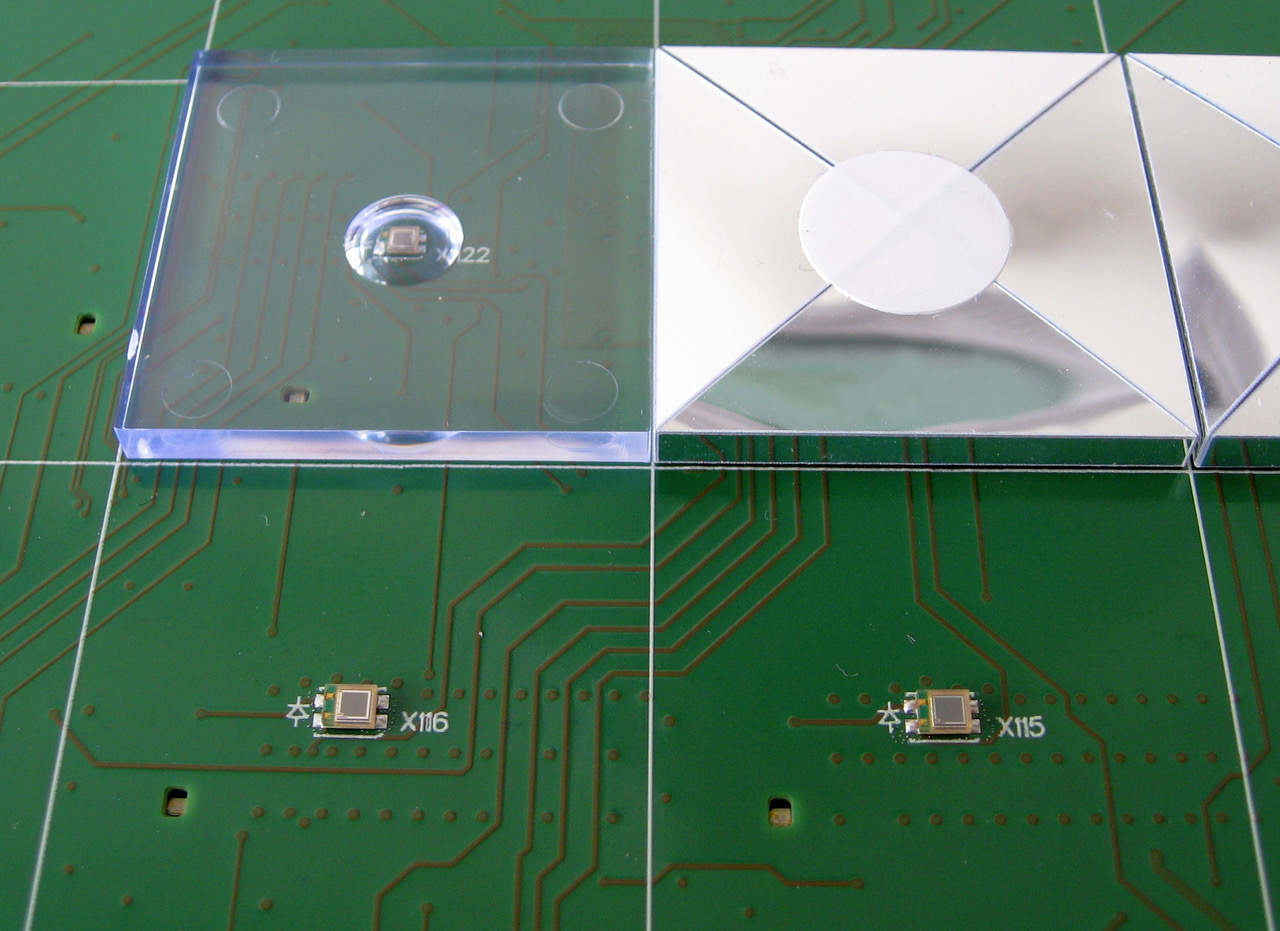
\includegraphics[width=0.39\textwidth]{Detector/fig/hcal-tiles.jpeg}
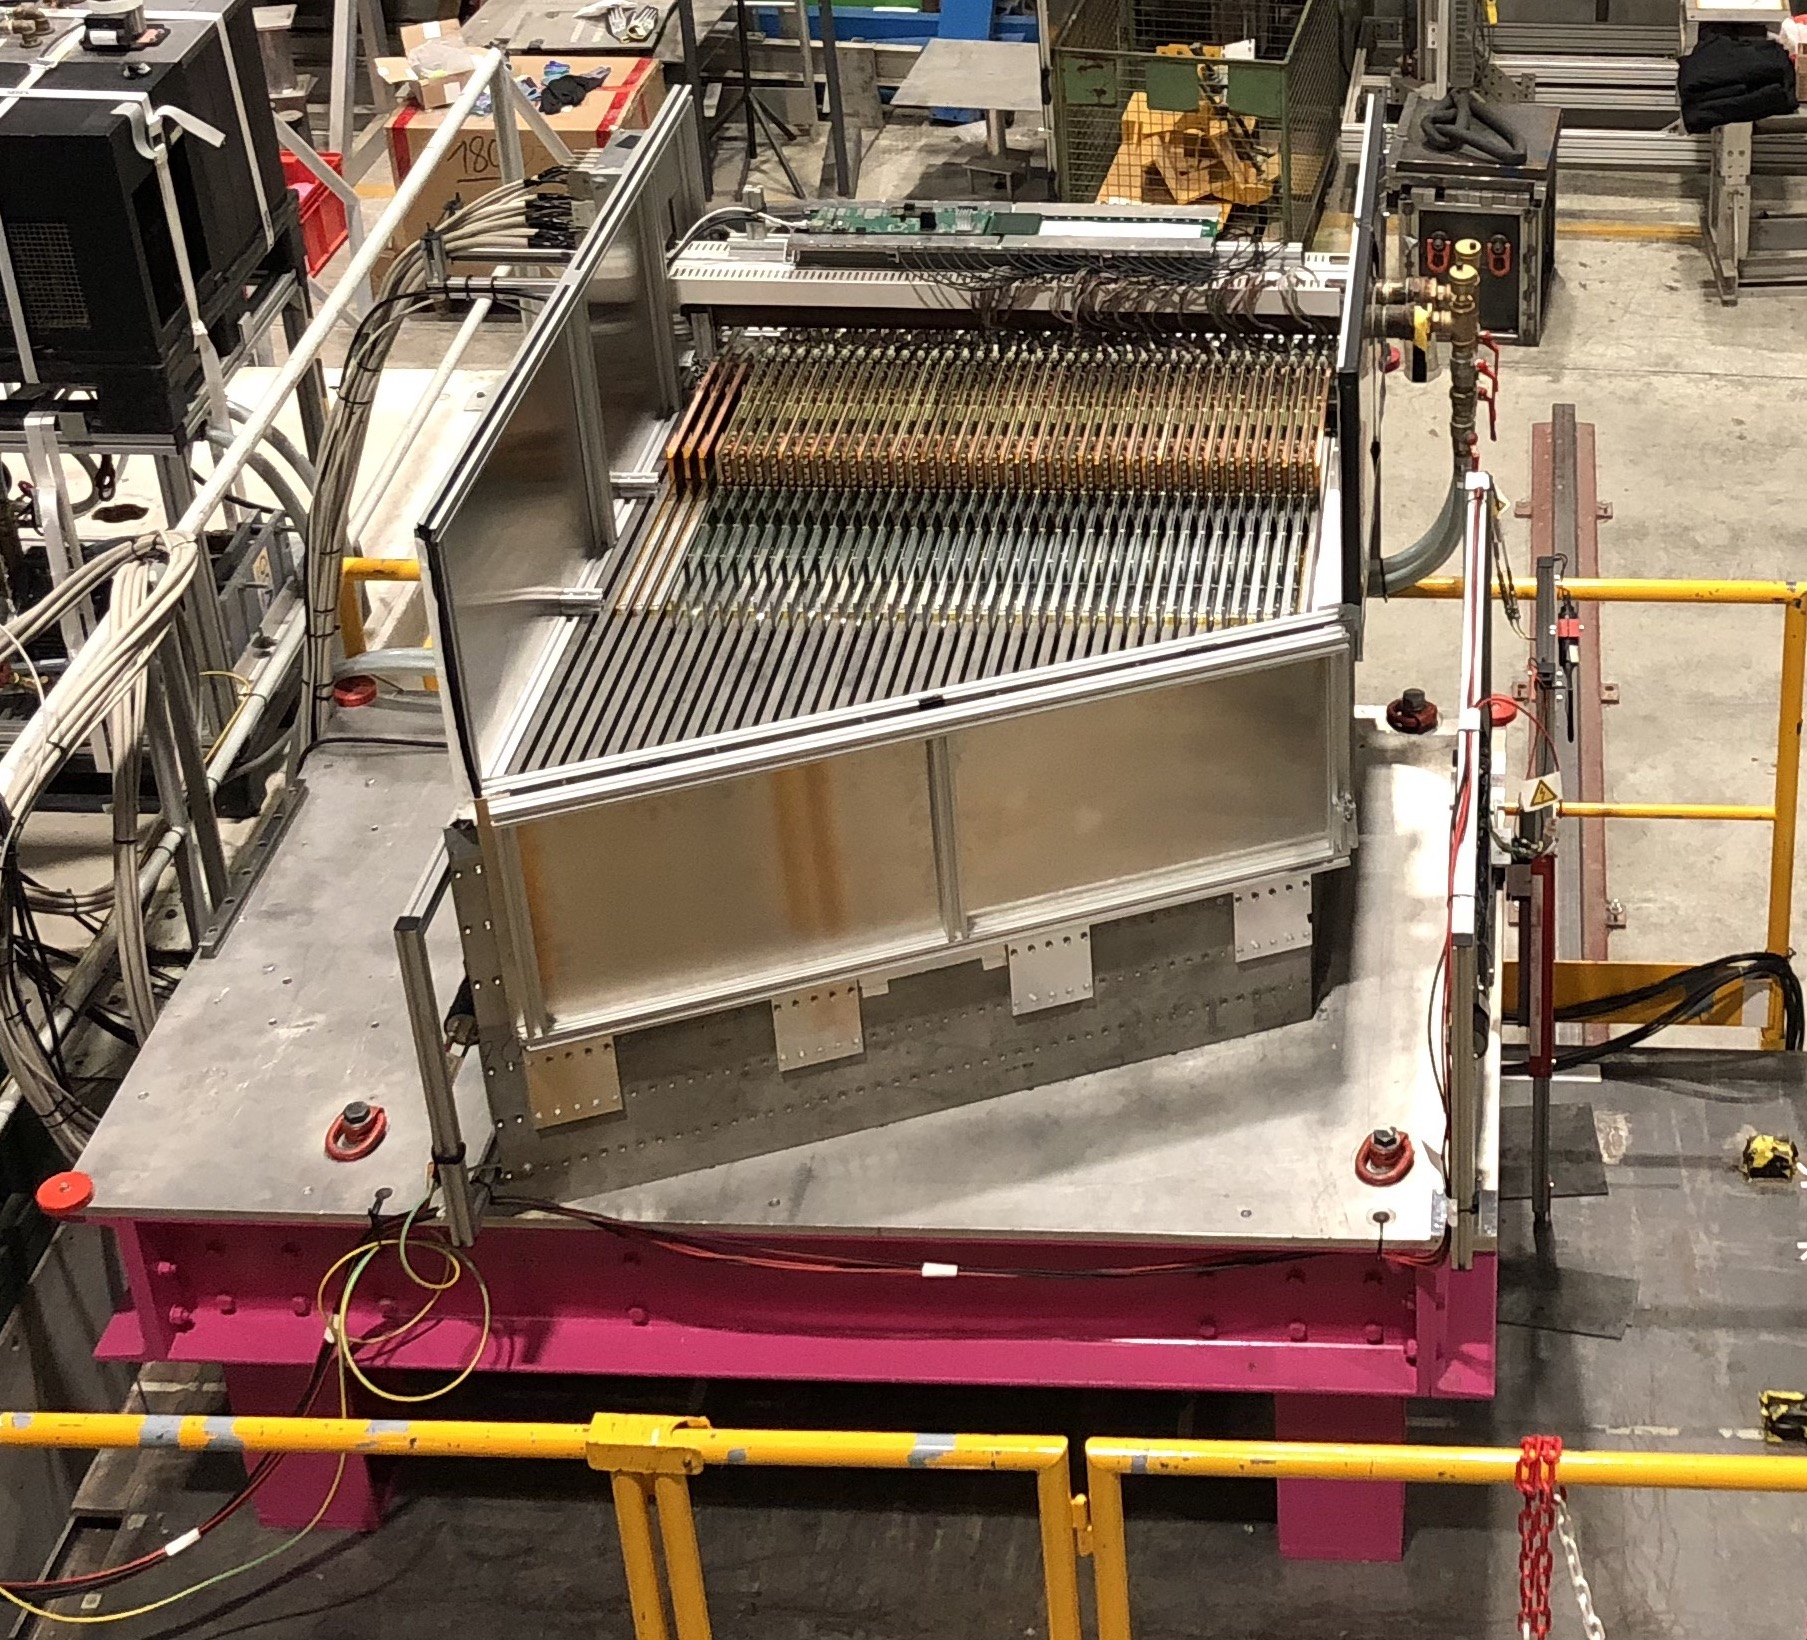
\includegraphics[width=0.59\textwidth]{Detector/fig/AHCAL-prototype.jpeg}
\caption{The AHCAL technological prototype. Left: Read-out board (HBU) with SiPMs and (un-)wrapped tiles. Right: Prototype installed in the H2 beam line at the CERN SPS.} 
\label{fig:AHCAL-TileProto}
\end{figure}
%
%The SiPMs were delivered in lots of 600 pieces with a uniform break-down voltage within $\pm 100$~mV. 
Spot-samples of all SiPM lots, and each one of the ASICs, had undergone semi-automatic testing procedures before soldering the HBUs \cite{Munwes:2634923}. The gain of the SiPMs was found to be uniform within~2.4\% when operated at a common over-voltage.
Without any further surface treatment, the scintillator tiles are wrapped in laser-cut reflective foil by a robotic procedure and mounted on the HBUs using a pick-and-place machine, after glue dispensing with a screen printer.   
%
The HBUs have been integrated into cassettes with interfaces for DAQ \cite{Kvasnicka:2017bpx}, LED pulsing and power distribution, which provide active compensation of temperature variations by automatic adjustments of the common bias voltage of the photon sensors in each layer. This was routinely used in test beam operation and stabilises the gain within $\pm 1\%$.
%Figure~\ref{fig:ActiveLayer} shows the top side of one active layer, with the scintillator tiles visible. 
%All layers have been  calibrated in the DESY test beam, and 99.96\% of the total 21888 channels are working.
%\begin{figure}
%\centering
%\includegraphics[width=0.7\textwidth]{figures/Layer-backside.jpg}
%\caption{Active layer side with wrapped tiles on 4 HBUs, with %\label{fig:ActiveLayer}
%\end{figure}
%
%The active layers were calibrated in the DESY test beam, assembled into the absorber stack and connected to 
Data concentration, power distribution and cooling service systems of the prototype are also scalable to the full ILD detector. 
%Figure~\ref{fig:AbsorberStructure} shows the active layers with connected services inserted in the absorber structure.
%\begin{figure}
%\centering
%\includegraphics[width=0.7\textwidth]{figures/AHCAL2.jpg}
%\caption{SiPM-on-tile AHCAL engineering prototype.}
%\label{fig:AbsorberStructure}
%\end{figure}

%The full prototype 
%has been commissioned with cosmic muons, exploiting its self-triggering capabilities and then
%; see Figure~\ref{fig:EventDisplay}.
%Two event displays are shown from cosmic rays interacting in the calorimeter. The top figures is a straight track from a minimum-ionising muon and the bottom is most likely a shower developed from an inelastic interaction of a muon with the absorber material.
The AHCAL technological prototype was installed in the test beam for data taking at the CERN SPS, see Fig.~\ref{fig:AHCAL-TileProto}.
During two periods in May and in June 2018, several $10^7$ events with muon tracks, as well as electron and pion showers in the energy ranges  10 -- 100~GeV and 10 -- 200~GeV, respectively, have been recorded. 
%The data taking rate averaged over the about 5~s long spills was up to 400 events per second.
Figure~\ref{fig:AHCAL-nhit-longslab} from the quasi-instantaneous data quality monitoring shows the distribution of the number of hits vs.\ the hit-energy weighted centre-of-gravity (cog) along the beam axis z for an electron run with a beam momentum of 100~GeV/c and admixtures of muons and hadrons. The different particle types populate different regions of the plot.
\begin{figure}[hbt]
\centering
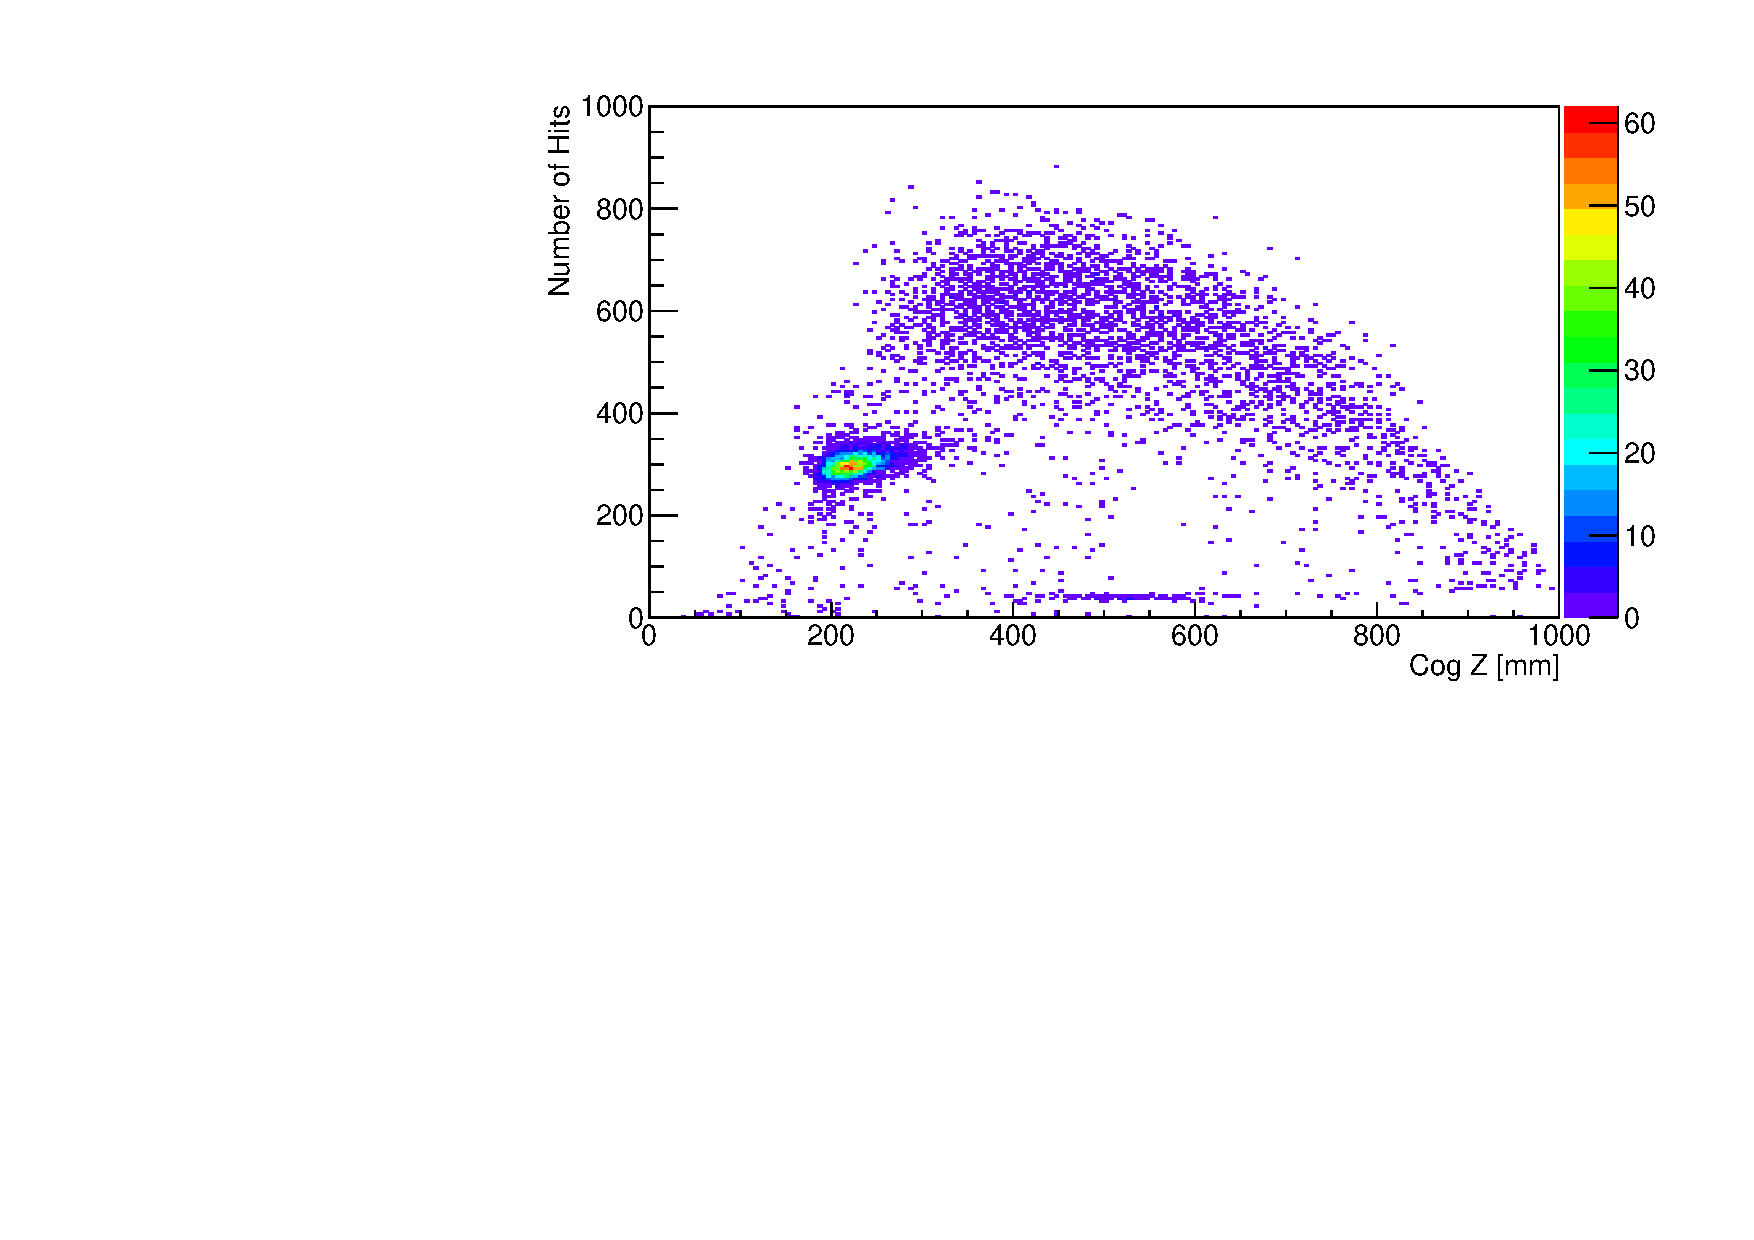
\includegraphics[width=0.64\textwidth]{Detector/fig/AHCAL-cogz_nhits.pdf}
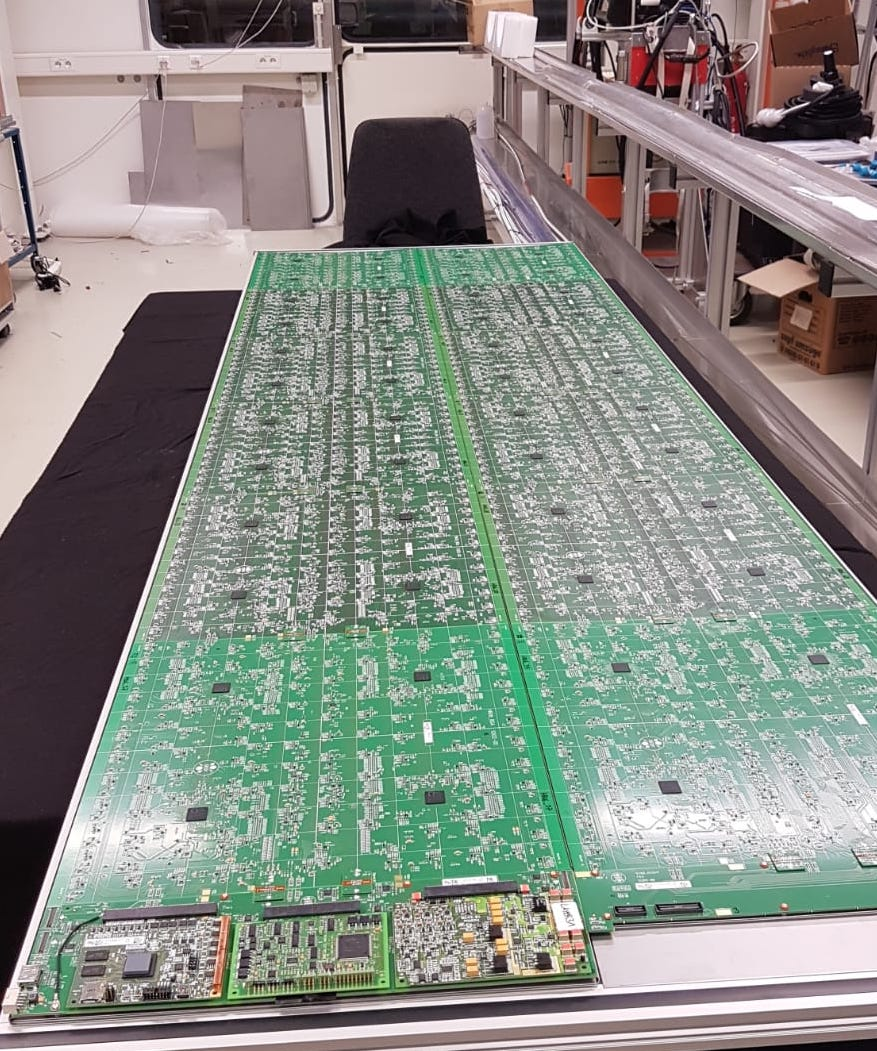
\includegraphics[width=0.34\textwidth]{Detector/fig/AHCAL-LomgSlab.jpeg}
\caption{Left: Distribution of the number of hits vs.\ the hit-energy weighted centre-of-gravity (cog) for a mixed beam in the AHCAL technological prototype. Right: Two slabs of HBUs with interfaces, corresponding to full ILD length in the TESLA configuration.} 
\label{fig:AHCAL-nhit-longslab}
\end{figure}
%
While electron showers are characterised by a relatively narrow distribution of number of hits and a cog near the front face of the detector, hadrons exhibit a wider distribution of the cog, and a larger number of hits, decreasing as the cog moves towards the rear of the detector, and leakage increases.
Muons appear as a narrow band with $\sim 38$ hits and a cog on z ay about half the depth of the detector. 

%The figure shows how the detailed topological information of the AHCAL can be used for the identification of particle types. The width of the distribution for electrons, and tails towards lower number of hits, suggest a compromised beam quality for the May period shown here, which indeed was resolved for the June period.
%
%\section{Conclusions}
%A highly granular hadron calorimeter prototype with 21888 channels, based on 3$\times$3~cm$^2$ scintillator tiles and SiPMs integrated with the embedded read-out electronics, has been successfully constructed and operated in test beams. The scalable design and automated construction and quality assurance procedures validate the concept for linear collider detector applications. 
%
The rich data sample collected in the two test beam periods in 2018  is being used for shower separation studies based on 5-dimensional reconstruction algorithms exploiting the high spatial, energy and time resolution of the prototype. 
While this is in progress, it can already be noted that in several aspects the  performance exceeds that of the physics prototype: the noise is a factor 100 lower, the dynamic range of the SiPMs is 3 times larger, and 99.96\% of the total 21888 channels are working.

The HBUs of the new prototype have also been used to build a large layer with two slabs of 6 HBUs each, corresponding to the full length of an ILD barrel sector in the TESLA layout, see Figure~\ref{fig:AHCAL-nhit-longslab}. The signal quality was unaffected, and the rise time of the power pulsing was within specifications. 

The AHCAL developments have also inspired the design of the scintillator section of the CMS end-cap calorimeter upgrade for the high luminosity phase of the LHC~\cite{Collaboration:2293646}, and the new prototype has been used together with silicon-instrumented sections in front in a common beam test, further illustrating the maturity of the technology. 
The new CMS endcap calorimeter will establish the SiPM-on-Tile technology in a collider environment at an intermediate scale between the AHCAL prototype and the full ILD detector. 

\subsubsection{RPC option (SDHCAL)}

The SDHCAL technological prototype built in 2011 has been regularly tested in beams in the past years with various configurations, including a combined test with the SiECAL prototype in 2018 (previous section). The SDHCAL prototype consists in 48 single-gap RPC layers of 1 $m^2$ (Figure~\ref{fig:det:SDHCAL_proto}). Each detection gap is instrumented with 6 Active Sensitive Units (ASU) made of a  50 x 33 $cm^2$ PCB with 24 "HARDROC" ASICs from OMEGA~\cite{Callier:2014uqa}. The RPC pad size is 1 $cm^2$ and the pad signals can be readout either in digital (1 bit and 1 threshold) or semi-digital (2 bits and 3 thresholds) modes.

\begin{figure}[t!]
\centering
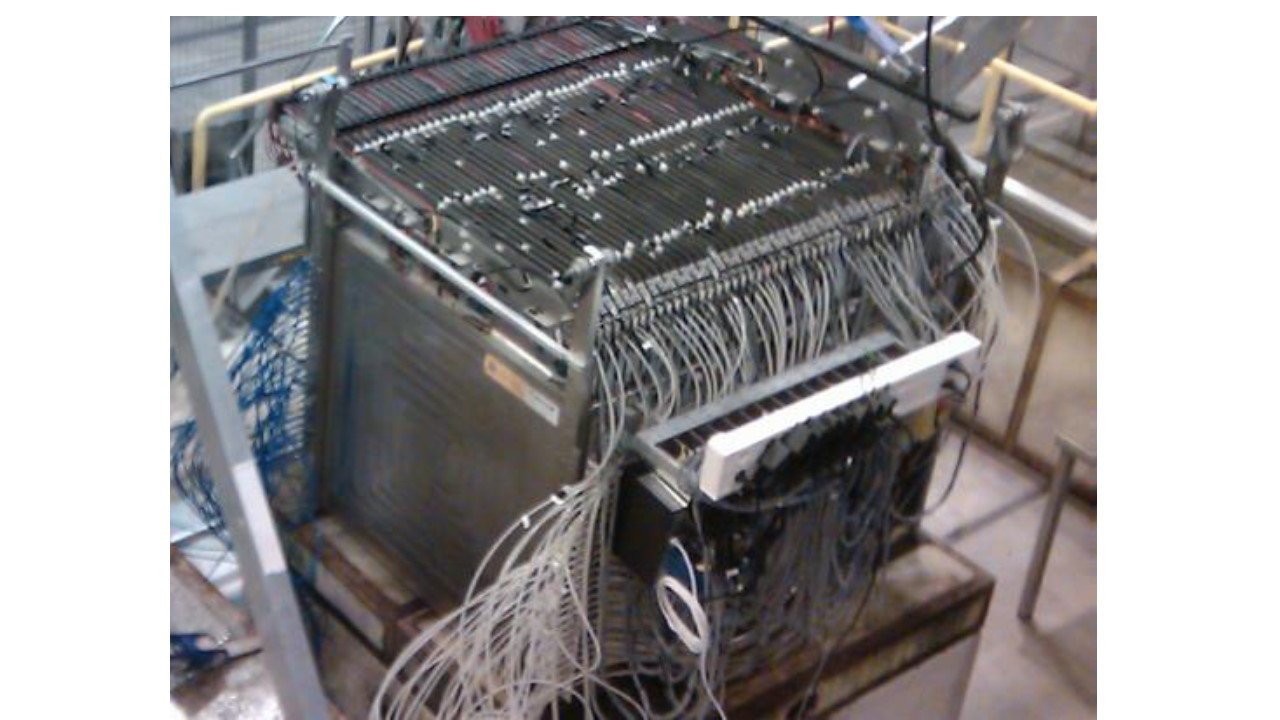
\includegraphics[width=0.8\hsize]{Detector/fig/SDHCAL_proto.jpg}
\caption{Technological prototype of the Semi-Digital Hadronic Calorimeter.}
\label{fig:det:SDHCAL_proto}
\end{figure}

The numerous data sets collected at CERN with high-energy hadron beams have been used to validate the performance of the technology. Special reconstruction methods adapted to the high granularity semi-digital structure of the calorimeter have been developed~\cite{Buridon:2016ill} to relate the energy estimation to the hit number and density. The current state of the performance is summarized in Figure~\ref{fig:det:SDHCAL_perf}. A good linearity is observed and the multi-threshold mode is found to mitigate saturation and improve the resolution at high energy. The description of the measured resolution by the simulation is however found to be sensitive to the description of the core of the hadronic showers, with a tendency for the Monte-Carlo to underestimate the performance due to harder cores in the showers~\cite{Deng:2016obt}. This point will require further tuning of the simulation.

\begin{figure}[t!]
\centering
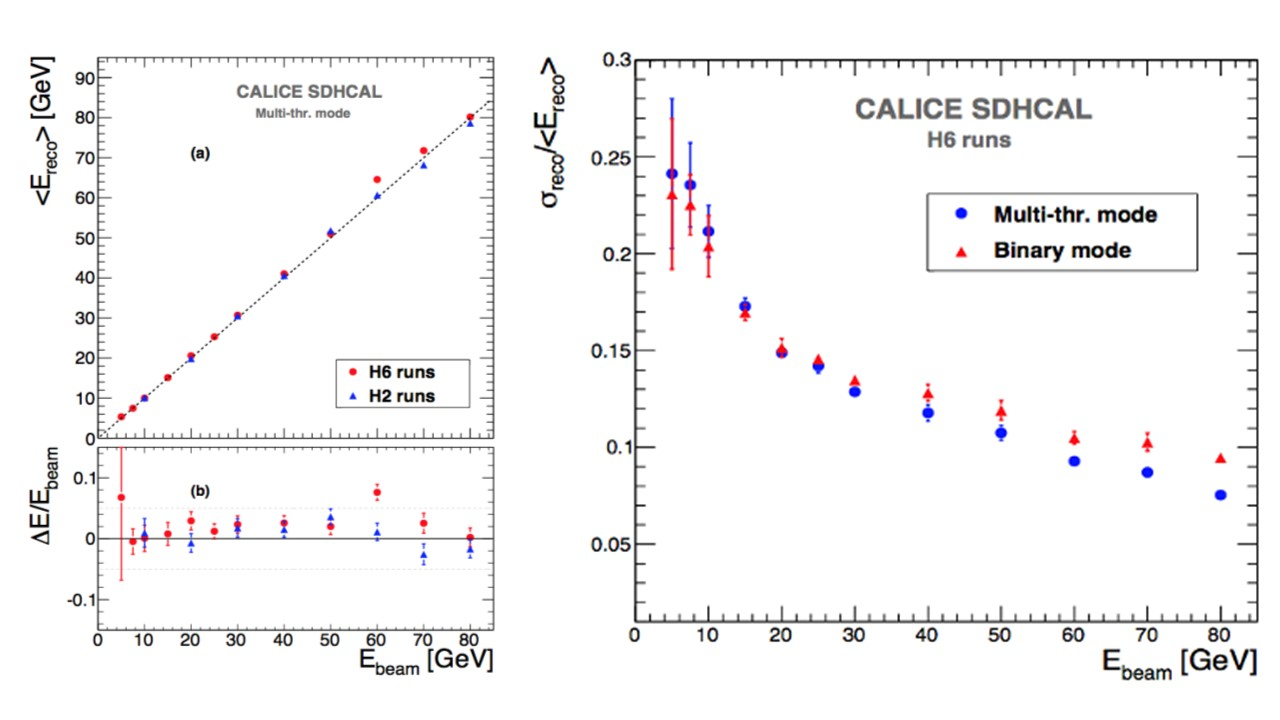
\includegraphics[width=1.0\hsize]{Detector/fig/SDHCAL_performance.jpg}
\caption{Performance of the SDHCAL technological prototype as measured in beam tests: linearity (left) and energy resolution for the digital and semi-digital readout options (right).}
\label{fig:det:SDHCAL_perf}
\end{figure}

In the recent years the SDHCAL teams have focused on adapting the technology to the full-size ILD requirements, in order to cover detection surfaces of up to 1 x 3 $m^2$ required by the ILD Hadronic Calorimeter in its "Videau" configuration (section 5.1.2). An improved RPC gas circulation system with better uniformity has been designed and validated with the construction of two large RPC's. Larger ASUs of 100 x 33 $cm^2$ have been designed with a new version of the HARDROC ASIC including 0-suppression (Figure~\ref{fig:det:SDHCAL_dev} left), and their interconnection improved to allow chaining of up to 9 ASUs. Efforts have also been invested in the manufacturing process of self-sustained hadron calorimeter structures with high precision mechanical tolerance as required by the RPC insertion. A method of "roller levelling" has been used to machine steel absorber plates with a high flatness. A high precision electro-welding has been used to built a first large size prototype of 4 calorimeter layers (Figure~\ref{fig:det:SDHCAL_dev} right) which has proven that gap size variations well below 1 mm can be reached on such large structures. 

For the longer term the option of multi-gap RPC's with a high timing resolution of $\approx$20 ps is prototyped based on the "PETIROC" ASIC~\cite{Fleury:2014hfa}. 

\begin{figure}[t!]
\centering
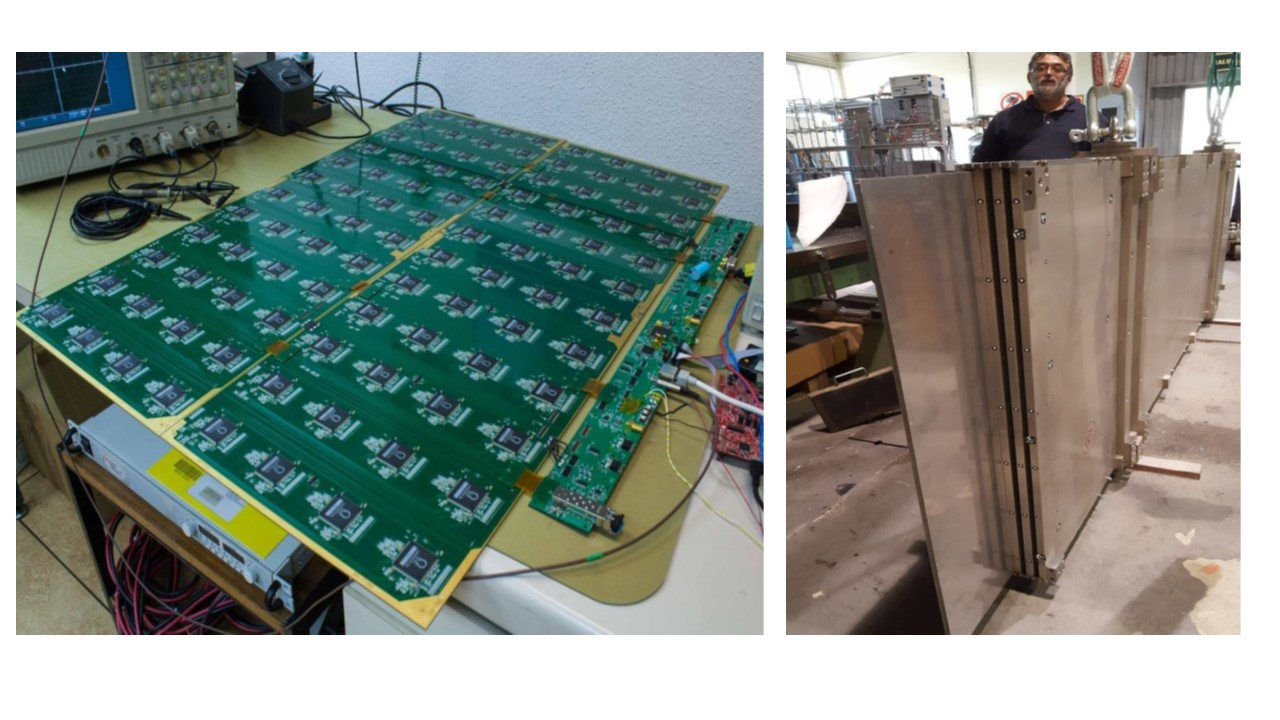
\includegraphics[width=1.0\hsize]{Detector/fig/SDHCAL_dev.jpg}
\caption{SDHCAL ongoing developments for the final ILD dimensions: two active sensor units of 100 x 33 $cm^2$ chained to each other and connected to the outside with a new compact DAQ interface (left), and self-sustained welded structure of 4 calorimeter plates of 1x3 $m^2$   with the required mechanical tolerances (right).}
\label{fig:det:SDHCAL_dev}
\end{figure}

\vspace{2cm}